% Befehl \fibelvorstellung: Erstellt die Vorstellung eines FSlers mit Bild
%	Parameter #1: Bild (wrapfigure)
%	Parameter #2: Text
\newcommand{\fibelvorstellung}[2]{%
	\begin{minipage}{\columnwidth}
		% Kein Abstand vor bzw. nach Bildern bei wrapfigure
		\setlength{\intextsep}{0cm}
		% geringfügiger Abstand zwischen Paragraphen
		\setlength{\parskip}{0.5ex}
		#1
		#2
		\vspace{0.5ex}
	\end{minipage}
	
	\vspace{5ex plus 2ex minus 1ex}
}
\newlength{\fibelstdlen}
\setlength{\fibelstdlen}{3.7cm}

\section{Der Fachschaftsrat~(FSR) Physik stellt sich vor}
\begin{multicols}{2}
\small


\fibelvorstellung{
	\begin{wrapfigure}{l}{0cm}
		\includegraphics[width=\fibelstdlen]{res/vorstellungsfotos/anna_niemann_cropped.PNG}
	\end{wrapfigure}
}
{Hey, ich heiße Anna und komm nun in mein drittes Mastersemester. Bei Fragen rund ums
	Studium und Münster könnt ihr mich gerne immer ansprechen.
	Wünsche euch einen wunderschönen Start ins Studium:)
}

\fibelvorstellung{
	\begin{wrapfigure}{r}{0cm}
		\includegraphics[width=\fibelstdlen]{res/vorstellungsfotos/benedikt_bieringer.png}
	\end{wrapfigure}
}
{Hallo zusammen! Mein Name ist Benedikt. In der Fachschaft beschäftige ich mich unter anderem mit Computergrafik/Design. Programmieren und Schwimmen sind nur zwei meiner weiteren Freizeitbeschäftigungen. In meinen mittlerweile schon 12~Semestern Fachschafts- und Studienerfahrung kann ich euch aber auch bei einer ganzen Reihe weiterer Fragen weiterhelfen.
}

\fibelvorstellung{
	\begin{wrapfigure}{l}{0cm}
		
\includegraphics[width=\fibelstdlen]{res/vorstellungsfotos/hauke_hawighorst.jpg}
	\end{wrapfigure}
}
{Moin, ich heiße Hauke und bin seit 2016 an der Uni und in der Fachschaft. Als Erasmus Student war ich in Sevilla (Spanien) und in Münster bin ich für die Evaluation der Lehre Zuständig. Euch ein herzliches Willkommen in Münster!
}


\fibelvorstellung{
	\begin{wrapfigure}{r}{0cm}
		\includegraphics[width=\fibelstdlen]{res/vorstellungsfotos/michael_te_vrugt}
	\end{wrapfigure}
}
{Hi, ich bin Michael und promoviere gerade in Physik und Philosophie. In der Fachschaft bin ich als Vorsitzender, Mitglied des O-Wochen-Teams und Beauftragter für alles mögliche immer gerne dabei. Bei Fragen zu Philosophie, einem Auslandsjahr, Doppelstudium oder Stipendium - und natürlich auch allem anderen - seid ihr bei mir genau richtig. Ansonsten wünsche ich euch viel Spaß in der O-Woche, und vielleicht sieht man sich mal bei einer Fachschaftssitzung :)}
	
\fibelvorstellung{
	\begin{wrapfigure}{l}{0cm}
		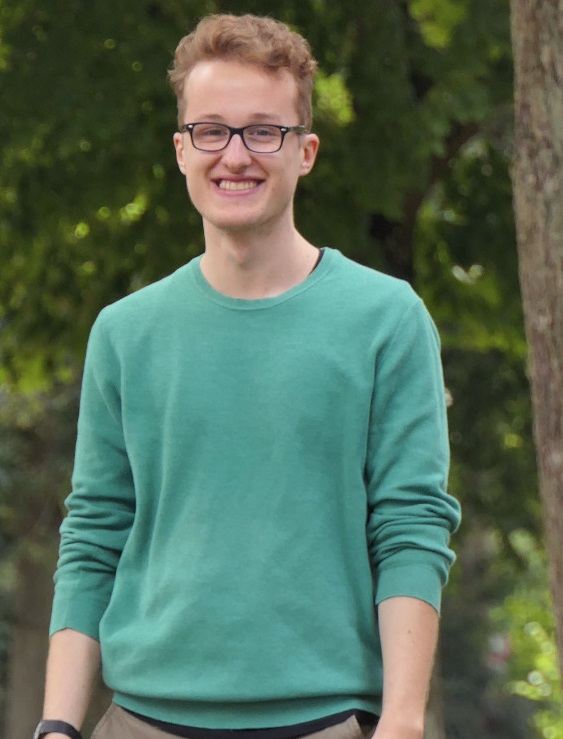
\includegraphics[width=\fibelstdlen]{res/vorstellungsfotos/jan_kirchner_neu.jpg}
	\end{wrapfigure}
}{
	Hallo! Ich bin Jan, seit Wintersemester 2016 in der Fachschaft, und vertrete uns auf der Fachschaftenkonferenz. Mittlerweile bin ich hauptsächlich im allgemeinen Studierendenausschuss aktiv. Ich kann euch sehr empfehlen, euch neben dem Studium auch in der Studierendenschaft einzubringen, und wünsche euch einen guten Einstieg in das erste Semester!
}

\fibelvorstellung{
	\begin{wrapfigure}{r}{0cm}
		\includegraphics[width=\fibelstdlen]{res/vorstellungsfotos/jan_honermann}
	\end{wrapfigure}
}
{Hi, ich bin Jan und sitze gerade an meiner Doktorarbeit. Falls ihr Fragen habt, könnt ihr euch gerne an mich wenden, ich bin meistens netter, als ich aussehe ;)
}
	
\fibelvorstellung{
	\begin{wrapfigure}{l}{0cm}
		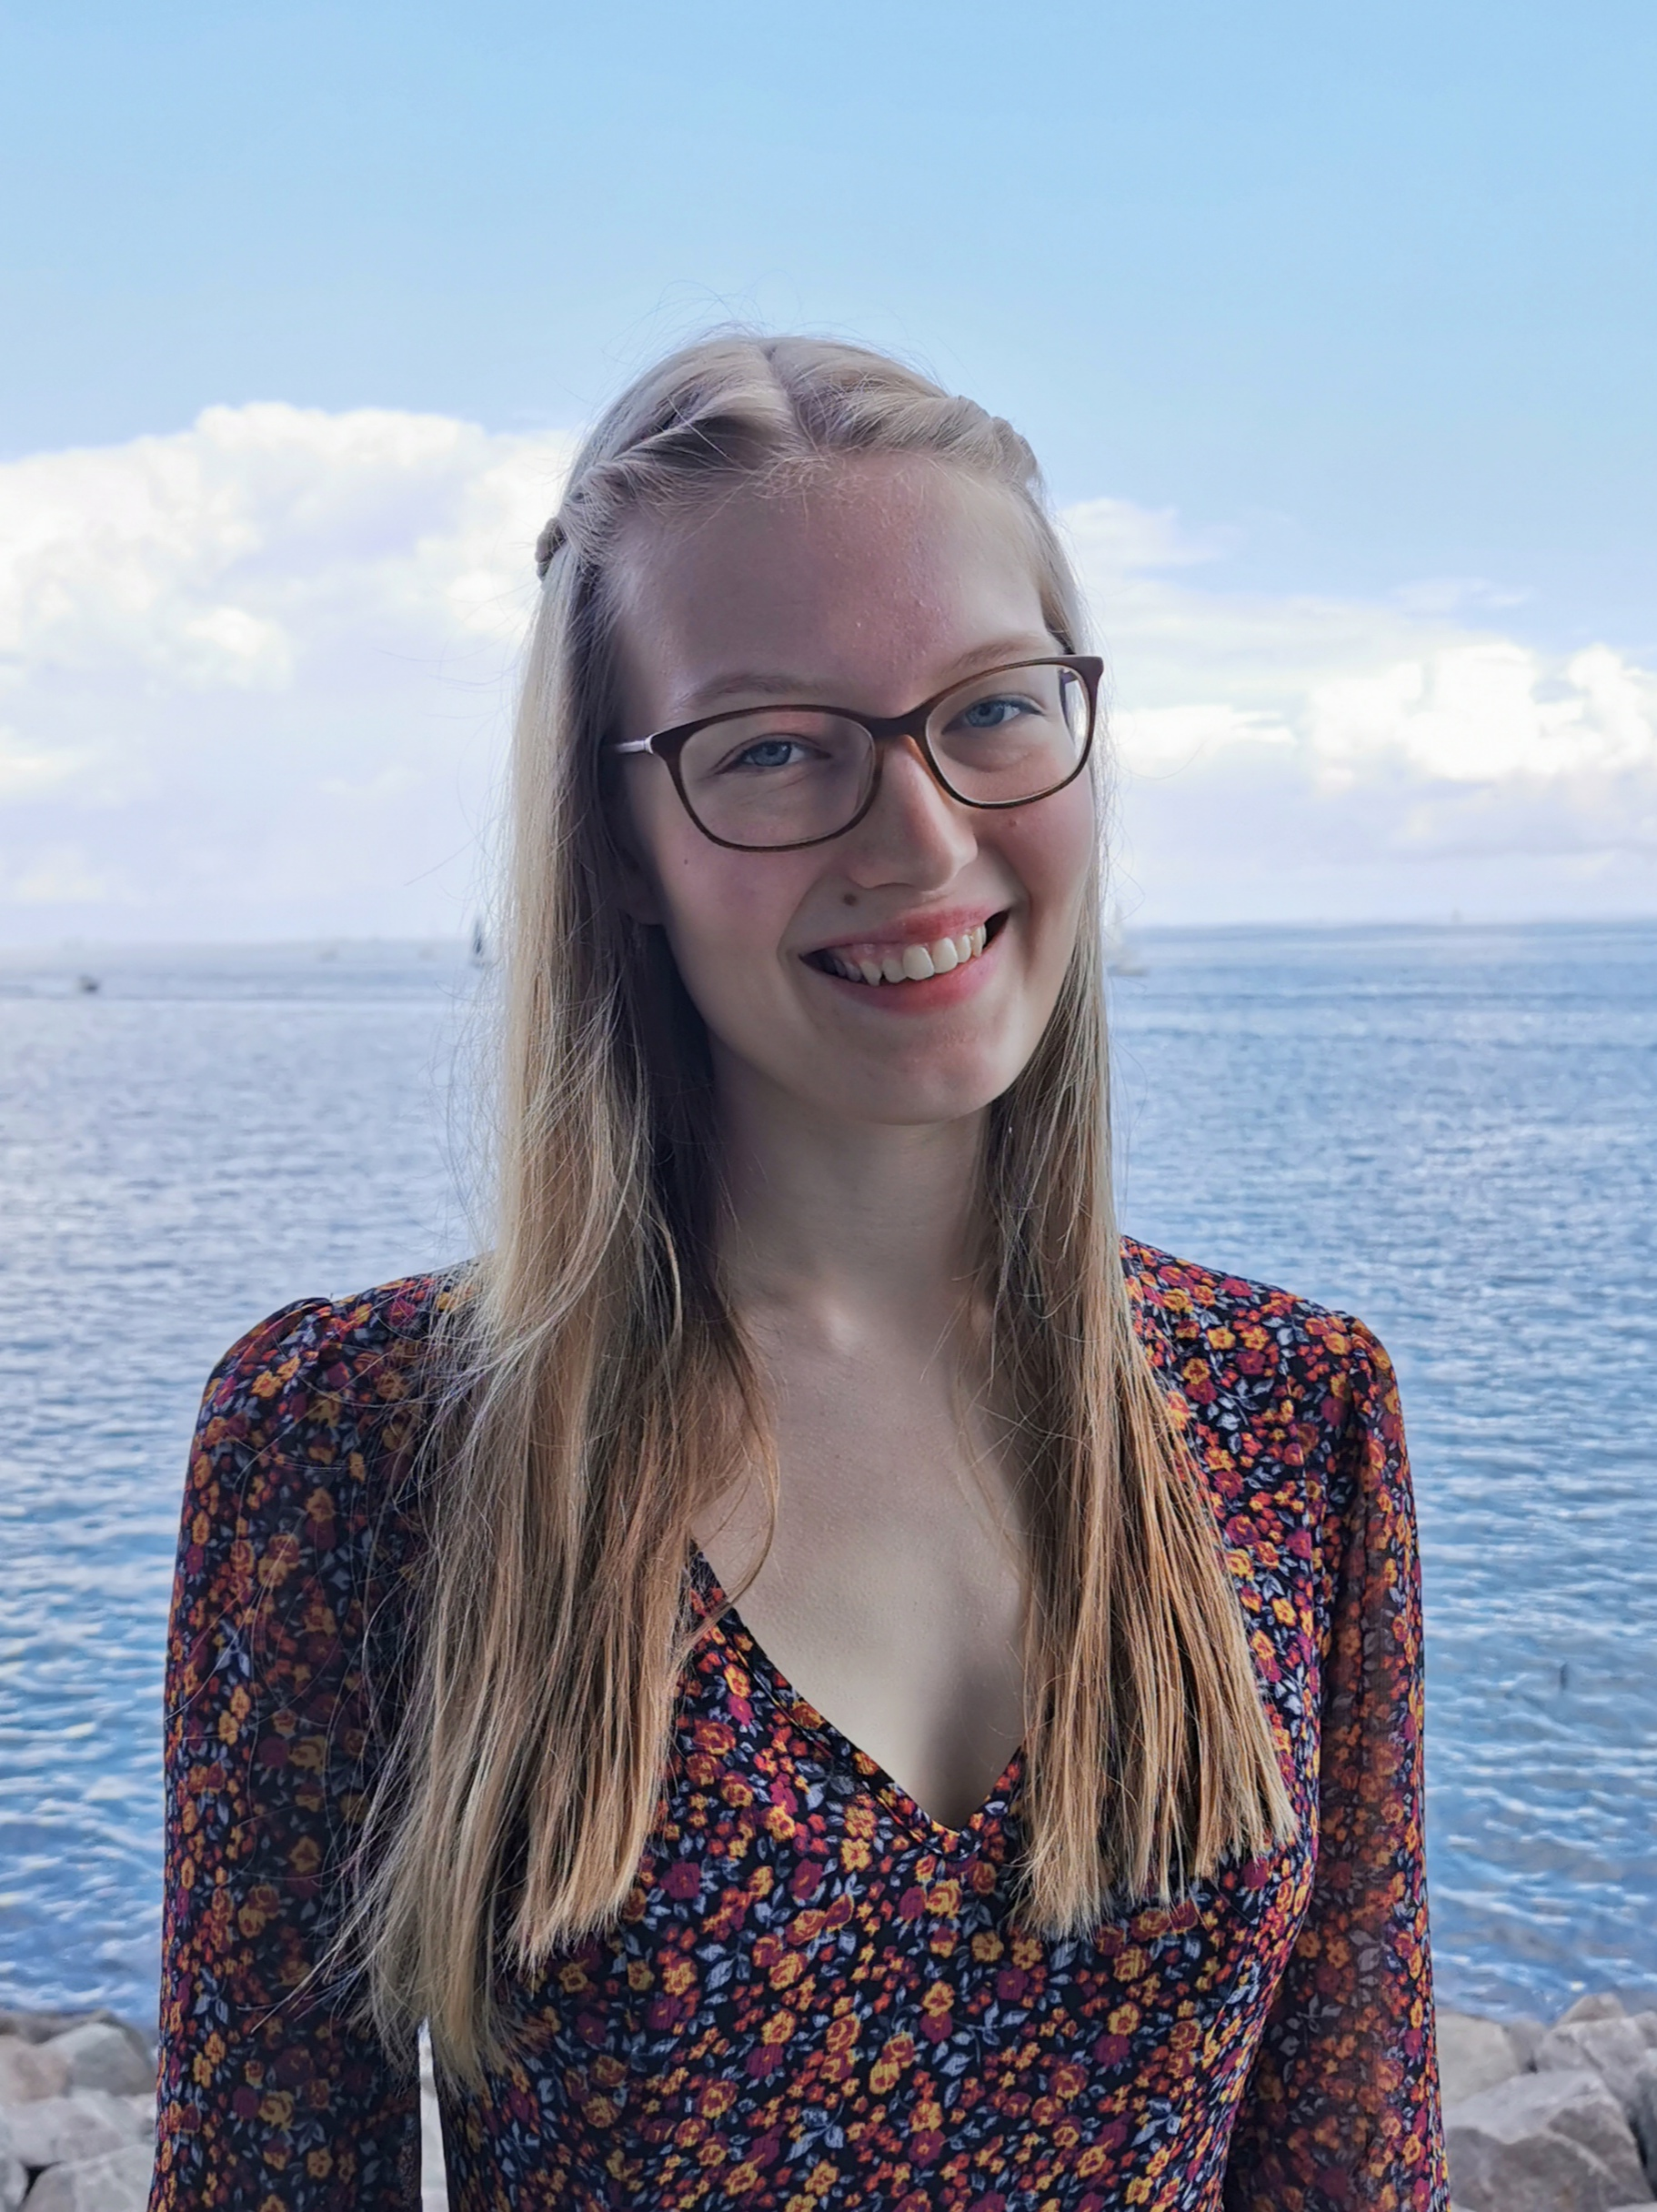
\includegraphics[width=\fibelstdlen]{res/vorstellungsfotos/paula_mors.jpg}
	\end{wrapfigure}
}{
Huhu, ich bin Paula und seit dem Sommersemester 2019 in der Fachschaft. Neben Fragen Rund um das Studium könnt ihr mich auch gerne auf royale Hochzeiten oder Filme mit Audrey Hepburn ansprechen. Ich wünsche euch einen lustigen Start ins Physikstudium!
}

\fibelvorstellung{
	\begin{wrapfigure}{r}{0cm}
		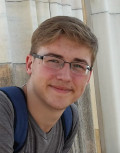
\includegraphics[width=\fibelstdlen]{res/vorstellungsfotos/christoph_wesseler.jpeg}
	\end{wrapfigure}
}{
Sehr geehrte Erstis: Moin!
Ich bin Christoph und studiere im 3. Semester Physik. In der Fachschaft bin ich im O-Wochen Team und beim Sommerfest tätig. Wenn Ihr Fragen habt, z.B zur O-Woche oder zum etwas Chaotischen Alltag an der Uni, immer her damit, es lebe das Chaos :D ich wünsche euch allen eine schöne O-Woche und hoffe man sieht sich mal in der Fachschaft.
}

\fibelvorstellung{
	\begin{wrapfigure}{r}{0cm}
		\includegraphics[width=\fibelstdlen]{res/vorstellungsfotos/kristin_nissen.jpg}
	\end{wrapfigure}
}{
Hey ihr lieben! Ich bin Kristin und nun im 5. Semester meines Physikbachelors. Ich kümmere mich in der Fachschaft um die Evaluation und auch um die Homepage. Falls ihr irgendwelche Fragen habt werde ich euch liebend gerne weiter helfen. Nun wünsche ich euch erstmal einen reibungsfreien Studienbeginn und viel Spaß in Münster.
}

\fibelvorstellung{
	\begin{wrapfigure}{l}{0cm}
		\includegraphics[width=\fibelstdlen]{res/vorstellungsfotos/marius_willer_cropped.jpg}
	\end{wrapfigure}
}
{Hi, ich bin Marius und heiße euch auch herzlich willkommen hier in Münster. Wenn ihr die Stadt noch nicht kennt, dann freut euch darauf, sie kennenzulernen. Das Studium wird zwar hart, aber lasst euch trotzdem nicht die Freude dran nehmen. ¡ Mucha suerte !}

\fibelvorstellung{
	\begin{wrapfigure}{r}{0cm}
		\includegraphics[width=\fibelstdlen]{res/vorstellungsfotos/lukas_eschmann_cropped.jpg}
	\end{wrapfigure}
}
{Moin liebe Erstis,
	mein Name ist Lukas und schon seit 2012 in der Fachschaft. Mein "normales" Studium habe ich bereits abgeschlossen, kann also so ziemlich alle Fragen zum Studium beantworten.
	Ich bin mittlerweile im Promotionsstudiengang angekommen und bin nur noch wenig in Hörsälen oder dem Fachschaftsraum anzutreffen.
	Auch Fragen zu Forschungsschwerpunkten der Uni oder aktuellen Themen der Forschung könnt ihr mir gerne stellen.}


%
% \begin{center}
% 	\includegraphics[width=\columnwidth]{res/fsphys_logo.pdf}
% \end{center}
%
%
%

\vspace{6ex}

\fibelvorstellung{
	\begin{wrapfigure}{l}{0cm}
		\includegraphics[width=\fibelstdlen]{res/vorstellungsfotos/fritz.png}
	\end{wrapfigure}
}
{Hallo, ich bin Fritz und bin neu in der Fachschaft Physik.
Die Mannschaft hier ist echt genial aufgestellt, sodass es richtigen Spaß macht, ein aktiver Teil der Universität Münster zu sein.
Ich kann dir nur empfehlen: Mach' mit und verändere die Uni!}
\end{multicols}

\vspace{20ex}

